\chapter{Background}\label{chp:background} 
\chapterprecishere{"We model the future on the past. Sometimes that’s a mistake."\par\raggedleft--- \textup{Van Jacobsen}, SIGCOMM 2001}

This chapter will give a brief overlook of the motivation for \gls{ICN},
as well as explaining more details of how \gls{ICN} protocols, such as \gls{CCN} and \gls{NDN}, works. 
It will also contain a quick summary of related works.

\section{Motivation for \gls{ICN}}
When Internet was created in the 1960's, the researchers where inspired by the existing communication network, the telecommunication network.
Because it was not natural and logical to think that people would download content, but rather send and receive short messages and instructions, the point-to-point communication model was a logical architecture. 
As Internet have developed, the traffic has increased enormously over the past few years. 
In the Global Internet Phenomena Report 1H2014 done by Sandvine~\cite{gipr2014}, close to 64\% of all \gls{IP} traffic in North America was Real-Time Entertainment streaming. 
In~\autoref{fig:ip-traffic} it can easily be seen that most of the traffic is content, and not communication.
With this in mind, the \gls{IP} architecture does not provide an efficient transport model for what we are actually using the network for.

\begin{figure}[ht]
  \centering
  \begin{subfigure}{0.48\textwidth}
    \centering
    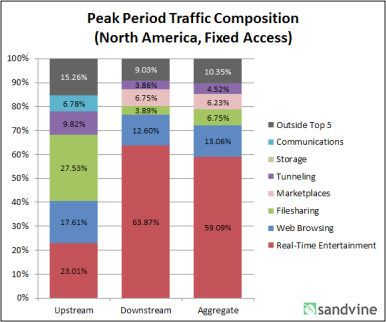
\includegraphics[width=1\linewidth]{north-america-ip-traffic.png}
    \caption{North America}
    \label{fig:north-america-ip-traffic}
  \end{subfigure}

  \begin{subfigure}{0.48\textwidth}
    \centering
    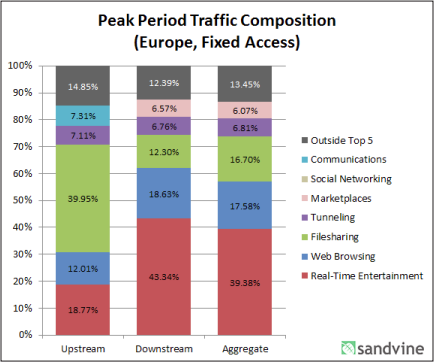
\includegraphics[width=1\linewidth]{europe-ip-traffic.png}
    \caption{Europe}
    \label{fig:europe-ip-traffic}
  \end{subfigure}
  \caption{
  (a) Peak Period Aggregate Traffic Composition - North America, Fixed Access~\cite{gipr2014}.
  (b) Peak Period Aggregate Traffic Composition - Europe, Fixed Access~\cite{gipr2014}.
  }
  \label{fig:ip-traffic}
\end{figure}

Also, the \gls{IP} network was not designed with security in mind. 
Most of the protocols related to Internet have been designed and deployed mainly with the goal of functionality to work.
\gls{IPsec} is a very good example of work trying to patch up security flaws in Internet.

A node in a \gls{IP} network does not know WHAT goes through, but rather the packet's endpoints, i.e. WHERE it goes and WHERE it comes from. 
This makes every node dumb, hence the network is designed for redundancy when it comes to content download.

\gls{TCP}/\gls{IP} not designed for broadcast and therefore wireless connection is not as easy as it can be.

These design failures are some the reasons why the research for Future Internet began.  
\gls{ICN}~\cite{DBLP:journals/cm/AhlgrenDIKO12} is a concept developed under this research.
It is built upon delivery of content, rather than the point-to-point model we previously have seen.
\gls{ICN}s goal is to build an infrastructure of a new Internet that can achieve efficient, secure and reliable distribution of content.
In 2012 \gls{IRTF} established \gls{ICN} working group.


\section{Content Centric Network \& Named Data Network}\label{chp2:sec:icn}
The first network protocol purposed for \gls{ICN}, \gls{CCN}, was presented by Van Jacobsen at Google Talk in 2006. 
He, amongst other contributors of \gls{CCN}, has been working on developing the Internet as we know since the early start.
Jacobsen has contributed to \gls{TCP}/\gls{IP}, i.a. with his flow control algorithms and \gls{TCP} header compression. 

\gls{CCN} focuses on naming content, instead of naming \gls{IP}-addresses. 
The research project is lead by \gls{PARC}.

A branch of \gls{CCN} is the \gls{NDN}~\cite{DBLP:journals/ccr/0001ABJcCPWZ14} research project started in 2010.
One of the biggest contributers is \gls{UCLA}, with Lixia Zhang in the lead.

\section{NDN Architecture}\label{chp2:sec:ndn_architecture}
Since the knowledge of how \gls{NDN} works is not disseminated amongst computer scientists, it is essential for this paper to describe how it works.
This section will describe the basic architecture of \gls{NDN} and compare some solutions with the equivalent solutions in \gls{IP}.

\subsection{Packets}
There is two types of packets in \gls{NDN};
\textit{Interest packet} and the corresponding answer, i.e. the \textit{Data packet}, illustrated in~\autoref{fig:packets}.
The Interest packet specifies a content name. 
The name has a hierarchical structure, e.g. ``/netflix/movie/1'' .  
An interest can also contain a selector that can be used to decide which data to satisfy the interest in case of multiple matches.
The Data packet it a response to the Interest packet, and contains the content for the name.
Now when somebody requests the movie ``/netflix/movie/1'' with an Interest, the response will have the same name, but also containing the movie. 

\begin{figure}[ht]
  \centering
  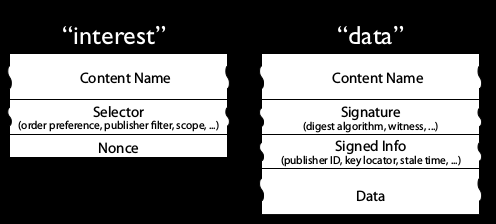
\includegraphics[width=1\textwidth]{packets.png}
  \caption{Packets}
  \label{fig:packets}
\end{figure}

Because only a Data packet can exists if there is a corresponding Interest, \gls{NDN} is pull-based.
This which means that there is no content in the network, that is not requested from someone.
This reduces unwanted traffic compared to \gls{UDP} in \gls{IP}.

\subsection{Node}
If we take a look at an existing model of an \gls{IP} node~\autoref{fig:ip-model-node} and comparing it to a \gls{NDN} node~\autoref{fig:icn-model-node}, they are very alike.

\begin{figure}[ht]
  \centering
  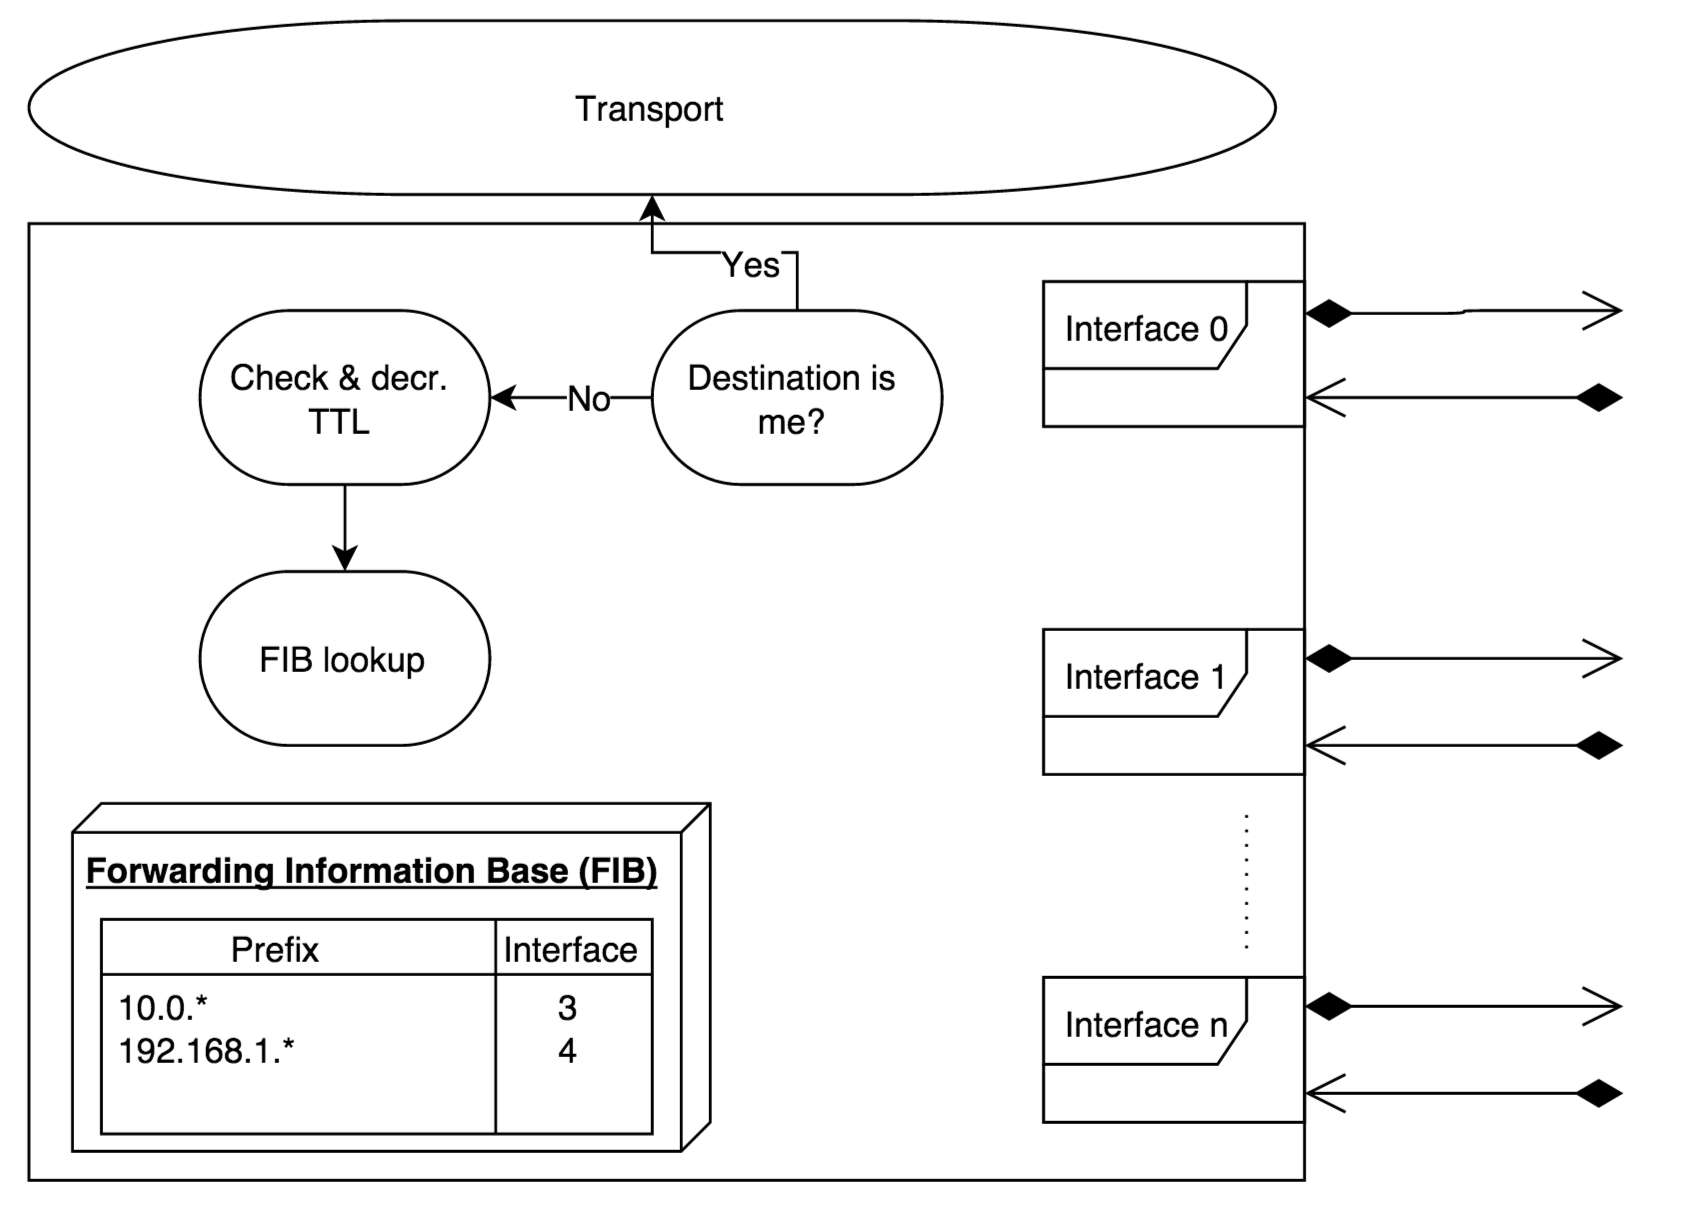
\includegraphics[width=1\textwidth]{ip_model_node.png}
  \caption{Model of \gls{IP} node. A packets enters the node through an interface. 
  The node decides whether the packet is for the node itself, or passes it further to next step, found in the \gls{FIB}.}
  \label{fig:ip-model-node}
\end{figure}

\begin{figure}[ht]
  \centering
  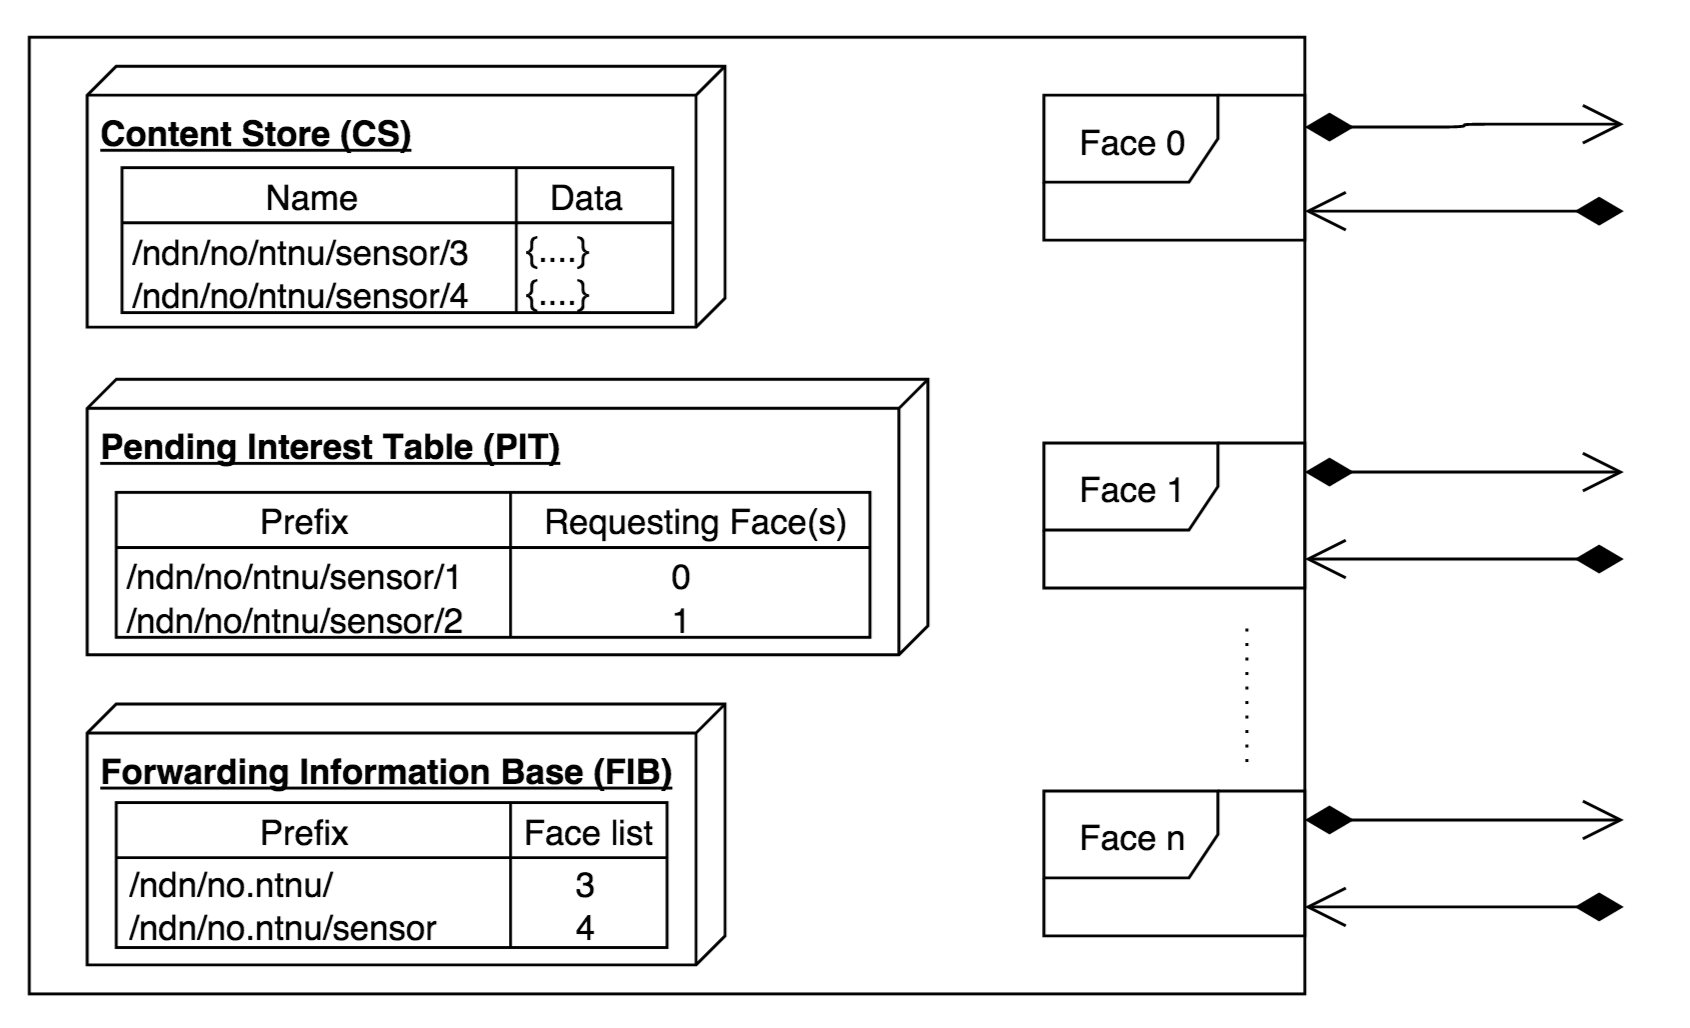
\includegraphics[width=1\textwidth]{icn_model_node.png}
  \caption{Model of \gls{NDN} node. A packet enters through an interface called Face. 
  The node checks whether the Interest is already queried in the \gls{PIT}, }
  \label{fig:icn-model-node}
\end{figure}

However, the logic behind a \gls{NDN} node is a bit more complex. 
In~\autoref{fig:icn-model-node-decision} we see that an incoming Interest.
\begin{figure}[ht]
  \centering
  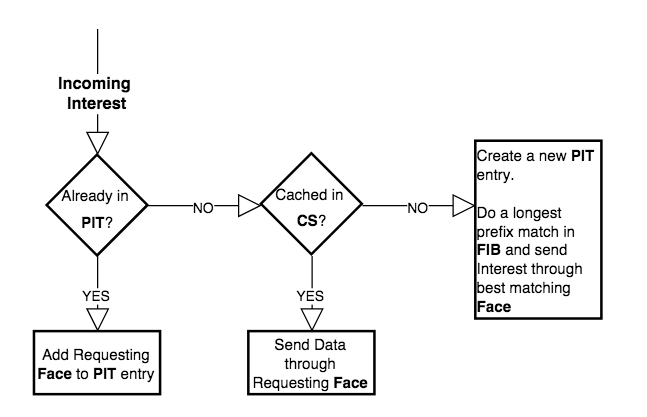
\includegraphics[width=1\textwidth]{ndn-node-decision-tree.png}
  \caption{Decision tree for a \gls{NDN} node when receiving an Interest.}
  \label{fig:icn-model-node-decision}
\end{figure}



Security aspects of the network protocol. 
The network demands that every packet delivered from application layer is signed by the application for integrity and authenticity.

Nodes know WHAT (name) they have. 
Nodes know what content they have, hence can share relevant data.

Face - an interface. Can be Ethernet, \gls{TCP}/\gls{UDP}, Websocket
strip away link layer headers (if any)

\subsubsection{\gls{PIT}}\label{pit}
\gls{PIT}~\autoref{fig:icn-model-node}- All pending or recently satisfied Interests are stored here, together with the incoming and outgoing interface.
If a new incoming Interest matches a entry in the \gls{PIT}, the incoming interface will be added to the entry. 


\subsubsection{\gls{CS}}\label{content-store}
\gls{CS}~\autoref{fig:icn-model-node} - When a node receives a Data packet that has a corresponding entry in the \gls{PIT}, it stores the data packet in the \gls{CS}. \gls{CS} is a cache of data packets.


\subsubsection{\gls{FIB}}\label{fib}
\gls{FIB}~\autoref{fig:icn-model-node} - Here a forwarding strategy is stored for each prefix. 
When a node forwards a Interest, it will do a longest prefix lookup in the \gls{FIB} and send the interest further to the best matching interface.


\subsubsection{\gls{RIB}}\label{rib}
\gls{RIB}~\autoref{fig:icn-model-node} - \todo{where?}

 
\subsection{Incoming Interest}
Incoming Interest through a interface (Face). The node checks the \gls{PIT} for pending or recently satisfied interests. 
If there is no match, the node will do a lookup in \gls{CS} to see if a corresponding Data packet is cached. 
If there is a match in the \gls{PIT} it will only add the interface to the \gls{PIT} entry. If there is a match in the \gls{CS} the node will return the Data. 
If there is no match in either the \gls{PIT} or the \gls{CS} the node will make a new \gls{PIT} entry and do a longest prefix match lookup in the \gls{FIB} to decide which interface to forward the Interest.
\todo{decision tree}

\subsection{Incoming Data}
The node will check  the \gls{PIT} for an entry, if match it will forward the data to all the interfaces registered in the \gls{PIT} entry.
Check data from local applications first cached in \gls{CS}, if not, store in \gls{CS} send data to all requesters (\gls{PIT})
\todo{decision tree}

\subsection{Outgoing Interest}
How to forward a Interest; routing strategy. A strategy per \gls{PIT} entry. I.e. whether, when, and where to forward Interest.
\todo{decision tree}

\subsection{Outgoing Data}
Send data through all interfaces registered in the \gls{PIT} entry. I.e. all requesters.
\todo{decision tree}

The architecture of \gls{NDN} is explained in detail in~\cite{NDN-0021}.

\subsection{Naming}\label{naming}
Naming is left to the application design.

\gls{DNS} naming
Email naming
\gls{OS} naming

\subsection{Anonymity}
Based on the nature of the architecture, \gls{NDN} facilitates the practice of anonymity in the network. 
Same concept as Tor network\todo{cite} and anonymity.
If a packet is captured at any arbitrary point of its path, the only information an adversary will get, is the two nodes between the packet capture and the data name. Unless monitoring a complete network, it should be close to impossible to track packets.  

Secure data VS secure channel

\section{Multicast By Nature}\label{ndn-multicast}

In~\autoref{fig:ndn-multicast} we can se that the network does not nearly have to send equal amount of traffic if every node is a \gls{NDN} node.
\begin{figure}[ht]
  \centering
  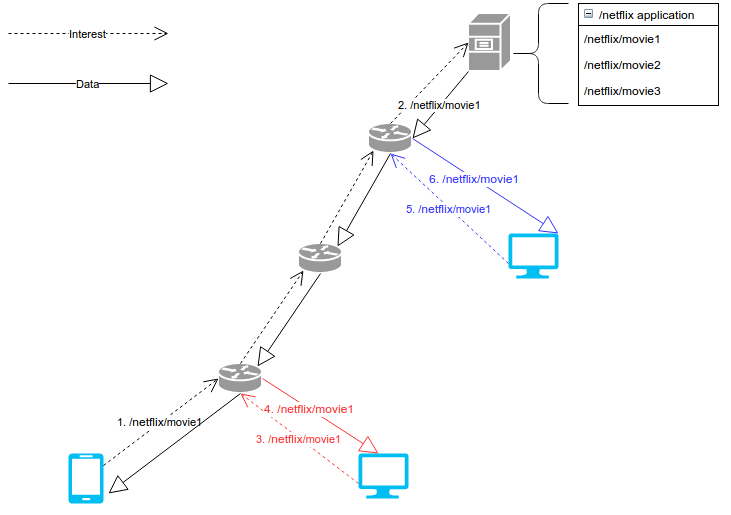
\includegraphics[width=1\textwidth]{ndn-multicast.png}
  \caption{Multicast in NDN.}
  \label{fig:ndn-multicast}
\end{figure}

\section{Attacks}

\subsection{Denial of Service attack}
Paolo Gasti et al. identifies several \gls{DoS} attacks on \gls{NDN} in their paper about \gls{DoS} \& \gls{DDoS} in \gls{NDN} ~\cite{DBLP:conf/icccn/GastiTU013}. 


modeling ddos~\cite{DBLP:journals/ijcomsys/WangCZQZ14}
Summary:


DDoS-resistant forwarding with hash tables~\cite{DBLP:conf/ancs/SoNO13}
Summary:


Mitigating Interest Flooding DDoS Attacks~\cite{DBLP:journals/corr/abs-1303-4823}
Summary:

\subsection{Cache attack}

Lightweight Integrity Verification and Content Access Control for Named Data Networking~\cite{DBLP:journals/tifs/LiZZSF15}
Summary:


Network-Layer Trust in Named-Data Networking~\cite{DBLP:journals/ccr/GhaliTU14}
Summary:


\section{Related work}
iSync~\cite{DBLP:conf/acmicn/FuAC14}
Summary:


Reliable retrieval of data from different wireless producers which can answer to the same Interest packet~\cite{DBLP:conf/acmicn/AmadeoCM14}
Summary:


Named data aggregation in wireless sensor networks~\cite{DBLP:conf/noms/AbidySLF14}
Summary:


Secure Sensing over Named Data Networking~\cite{DBLP:conf/nca/BurkeGNT14}
Summary: